\section{M\~aori Parts of Speech}

\subsection{Performance Results}

\begin{figure}[H]
  %  minipages
  \centering
  \begin{minipage}[b]{0.8\textwidth}
    \centering
    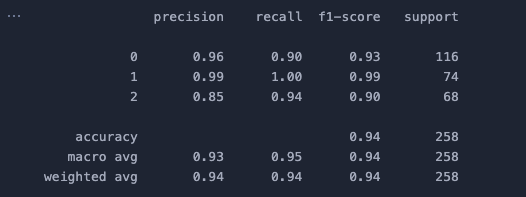
\includegraphics[width=0.9\textwidth]{figures/1-f1-1.png}
    \caption{M\~aori Parts of Speech}
    \label{fig:maori-pos-1}
  \end{minipage}
  \hfill
  \begin{minipage}[b]{0.8\textwidth}
    \centering
    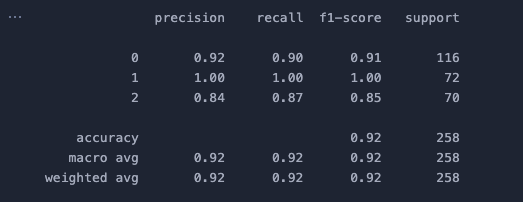
\includegraphics[width=0.9\textwidth]{figures/1-f1-2.png}
    \caption{M\~aori Parts of Speech}
    \label{fig:maori-pos-2}
  \end{minipage}
  \begin{minipage}[b]{0.8\textwidth}
    \centering
    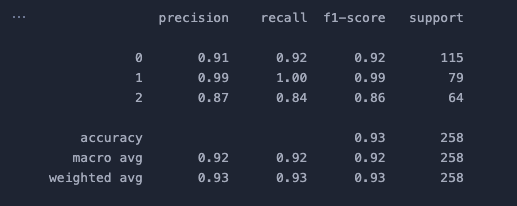
\includegraphics[width=0.9\textwidth]{figures/1-f1-3.png}
    \caption{M\~aori Parts of Speech}
    \label{fig:maori-pos-3}
  \end{minipage}
\end{figure}


\subsection{Notable Observations}

\begin{enumarabic}
  \item There is some variance in the \verb|F1| scores for the different parts of speech.
    This is because of how \verb|torch| randomizes the initial weights of the neural network.
    There is also some randomness in how the data is split into training batches and testing set,
    which affects the learned performance of the model.
  \item The \verb|F1| scores are consistently higher for certain parts of speech
    ($1 >> 0 >> 2$ in all three cases).
    This can be a result of the distribution of the data in the training and testing sets
    --- if one class has more examples or simpler identifiers
    then the model will learn to predict it better.
\end{enumarabic}
